\documentclass{article}   


\usepackage{url}    
\usepackage{natbib}
\usepackage{graphicx}
\usepackage{placeins}
\usepackage{tabularx,ragged2e,booktabs,caption}
\usepackage{amsmath}
\usepackage{lscape}
\usepackage{hyperref}
\usepackage[margin=1in]{geometry}
\usepackage[none]{hyphenat}


\begin{document}


\title{Moist Adiabats: Quest for Analytic Solution v2.0}
\author{Nadya Moisseeva}
\date{November 2015}    % type date between braces

\maketitle
% \tableofcontents

\newpage
\section*{Overview}
This document is intended to summarize the proposed approach to analytical modelling of moist adiabats. The current summary offers a simple (but rather inelegant) answer to: \emph{How can we determine temperature $T$, given pressure $P$ and moist adiabat $\Theta_w$?}

\FloatBarrier
\section*{Problem Setup}
The preliminary steps follow the solution originally suggested by R.Stull, with several modifications introduced to increase the precision of directly calculated moist adiabats. The following changes were made to the original method:
\begin{itemize}
\item{adjusted several constant values, including adjusted Clausius-Clayperon constant (Koutsoyiannis 2011)}
\item{replaced original Clausius-Clayperon relation with updated formula (Koutsoyiannis 2011)}
\item{introduced temperature-dependent latent heat of vaporization constants}
\item{introduced alternative $\Theta_e$ formula}
\item{increased pressure range to the top of the atmosphere (1kPa)}
\item{decreased pressure calculation step to 0.001 kPa}
\item{increased temperature range to -40C - 40C}
\end{itemize}

A sample of the resultant curves can be seen in Fig.~\ref{stuve}. Following Stull's original approach, moist adiabats can be normalized using equivalent potential temperature $\Theta_e$ and dry potential temperature $\Theta_d$, to produce a set of curves shown in Fig.~\ref{norm_theta}. From this point, Stull's solution attempts to normalize the pressure range, such that the curves collapse into a single shape. Based on the current investigation, it appears that the nature of the underlaying nonlinearity in the problem doesn't lend itself to such direct normalization. Hence, the current solution proceeds on a different path described below. 

\begin{figure}
\centering
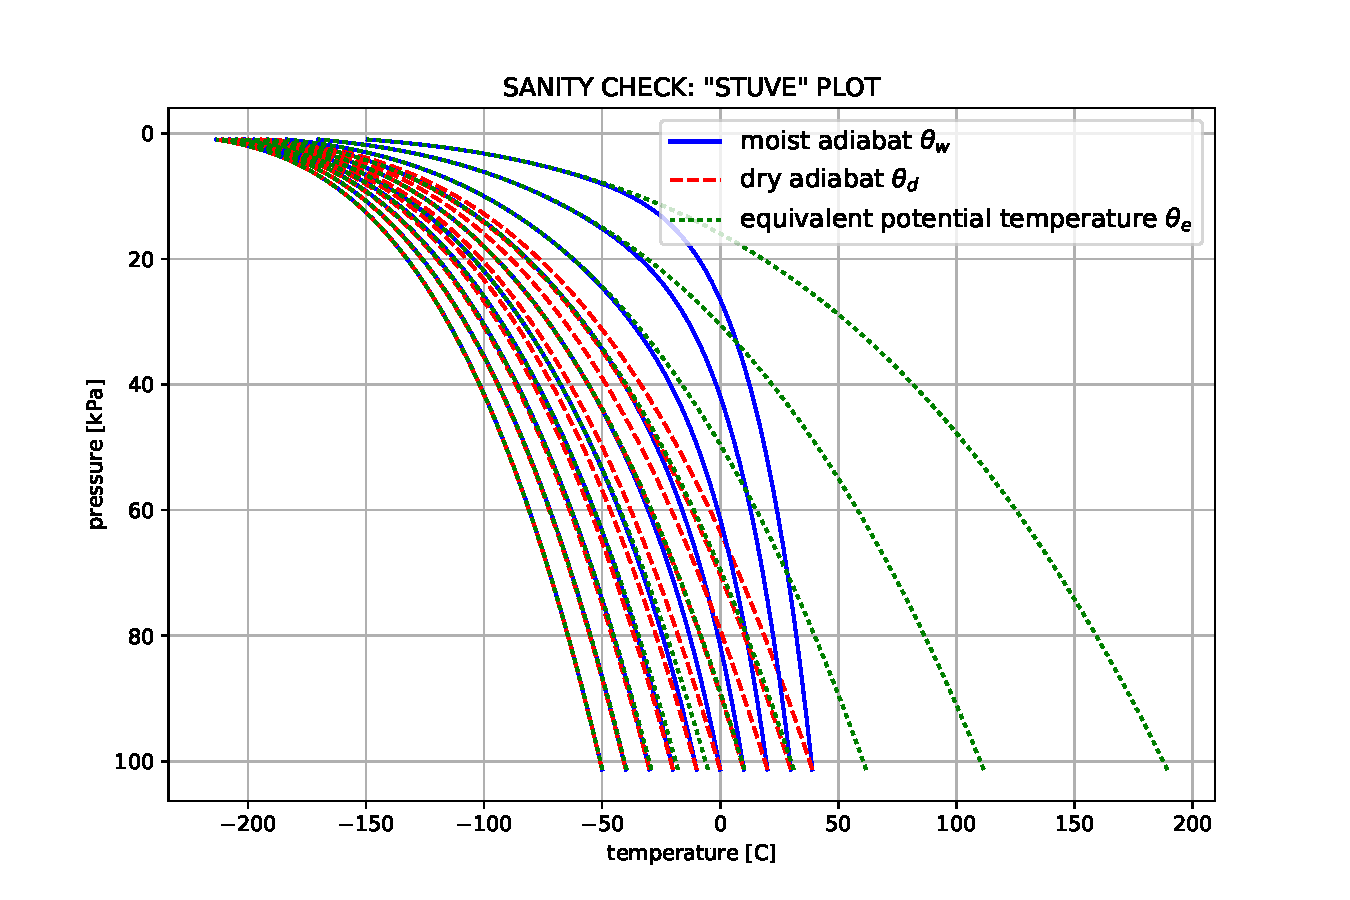
\includegraphics[width=4.5in]{../figs/stuve.pdf}
\caption{Directly calculated curves for moist adiabats, potential and equivalent potential temperatures. Limited temperature range shown. }\label{stuve}
\end{figure}

\begin{figure}
\centering
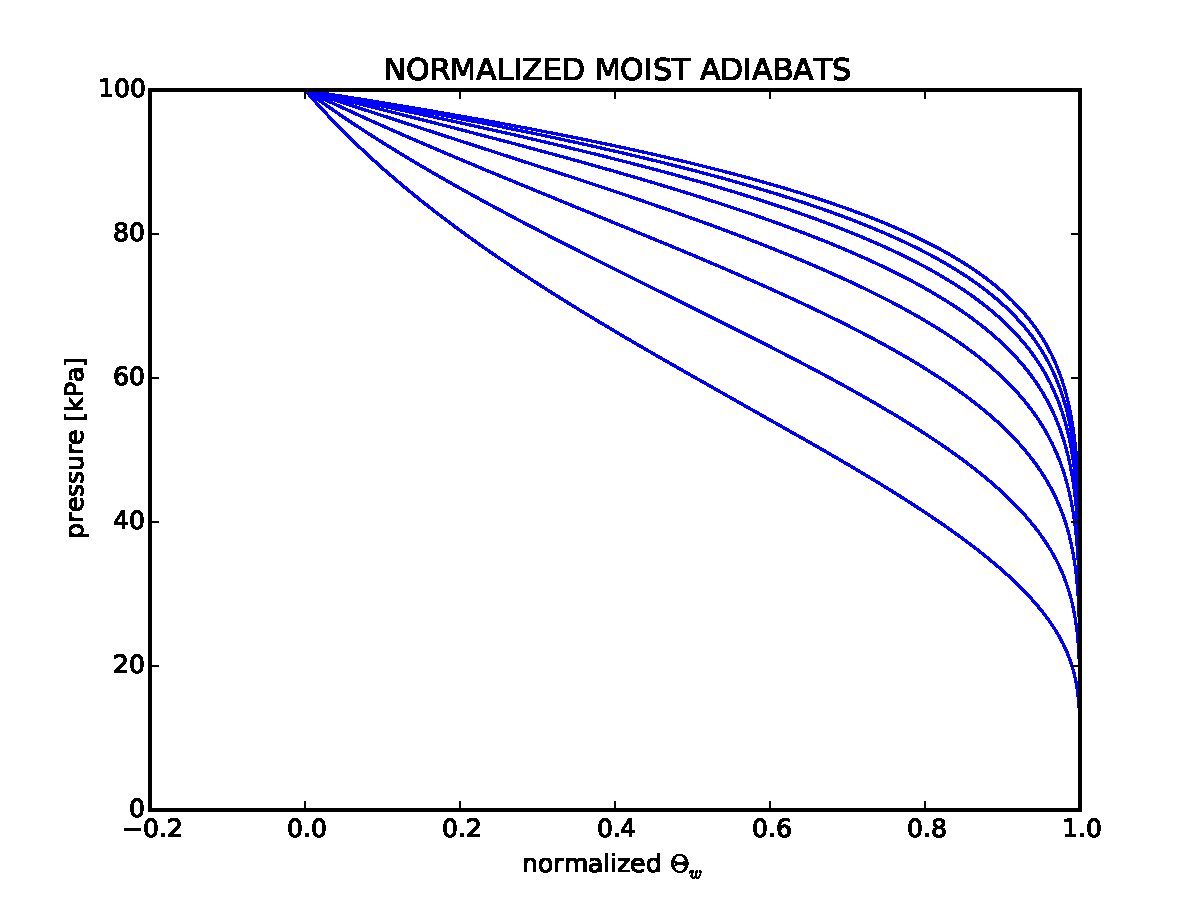
\includegraphics[width=4.5in]{../figs/norm_theta.pdf}
\caption{Normalized moist adiabats, following R.Stull. Select curves shown. }\label{norm_theta}
\end{figure}

\FloatBarrier
\section*{Modelling the Effects of Pressure on Normalized Curves}
The first step of the current solution attempts to remove some of the inherent nonlinearity by further normalizing the set of curves shown in Fig.\ref{norm_theta}. By choosing one of the normalized adiabats to represent a pressure reference curve $P_{ref}$, Fig.\ref{norm_theta} can be reduced to Fig.\ref{trans_adiabats}. The transformed adiabats shown are produced using a normalization with $P_{ref} = +40C $. This particular choice of $P_{ref}$ does not imply its theoretical importance. It is possible to choose any of the directly calculated normalized adiabats to represent $P_{ref}$. Depending on the choice, the resultant transformed adiabats will shift around the $P_{ref}$ unity line. The single consideration for choosing a particular $P_{ref}$ is the availability of simple analytical function that can represent all of the transformed curves. 

\begin{figure}
\centering
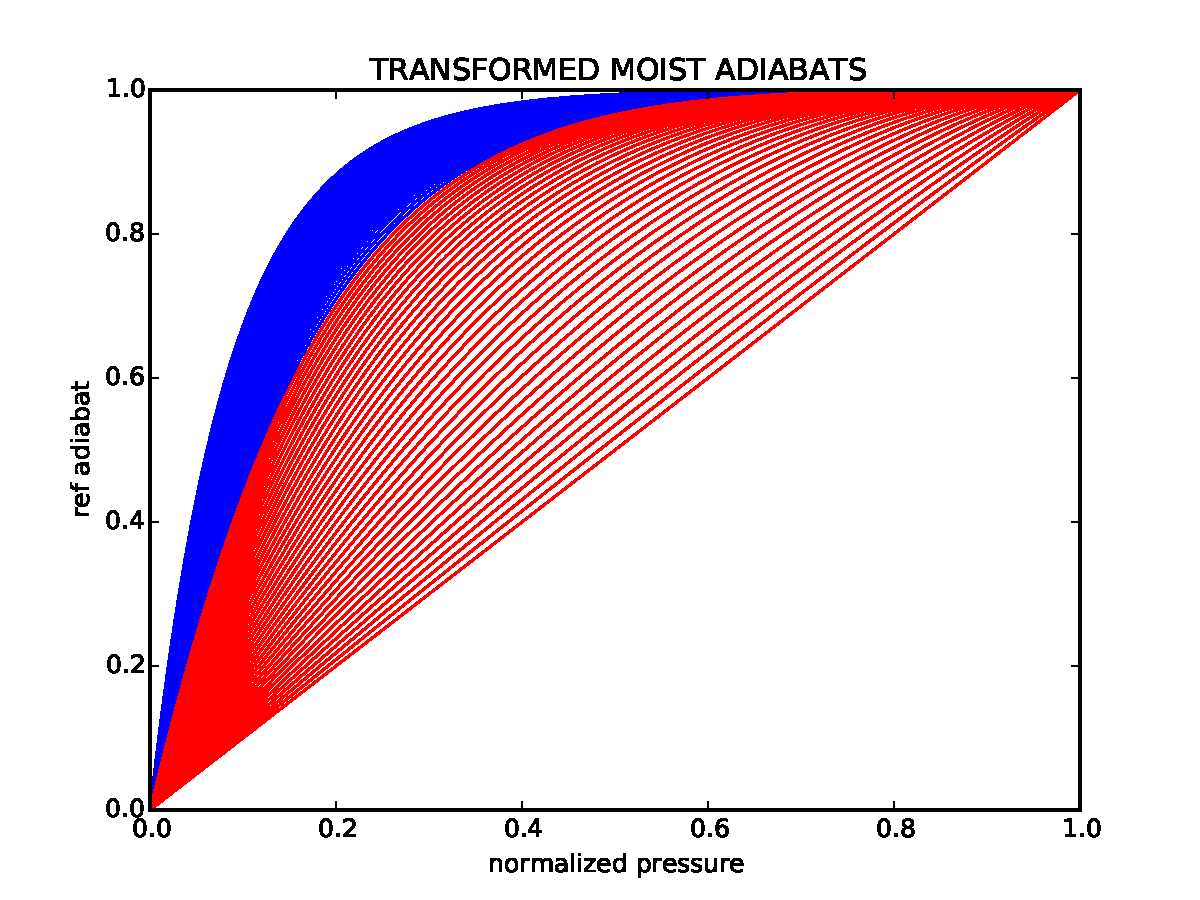
\includegraphics[width=4.5in]{../figs/trans_adiabats.pdf}
\caption{Transformed normalized adiabats. Colors correspond to negative (blue) and positive (red) temperatures.}\label{trans_adiabats}
\end{figure}

$P_{ref}$ can easily be modelled analytically using polynomial functions. This is convenient, since polynomials are generally well-behaved functions. The choice of the degree of polynomial depends on the desired precision level. Since we are examining a fixed range of temperatures relevant to atmospheric applications, the potentially chaotic behavior of high degree polynomials outside of the modelled range is not a primary concern. For this example, an extremely high accuracy threshold was chosen: the aim was to ensure that the mean average error (MAE) is on the order of $1x10^{-5}$. The true and modelled $P_{ref} = +40C$ can be seen in Fig.\ref{pref}. The fit was produced using a 28th degree polynomial. 

\begin{figure}
\centering
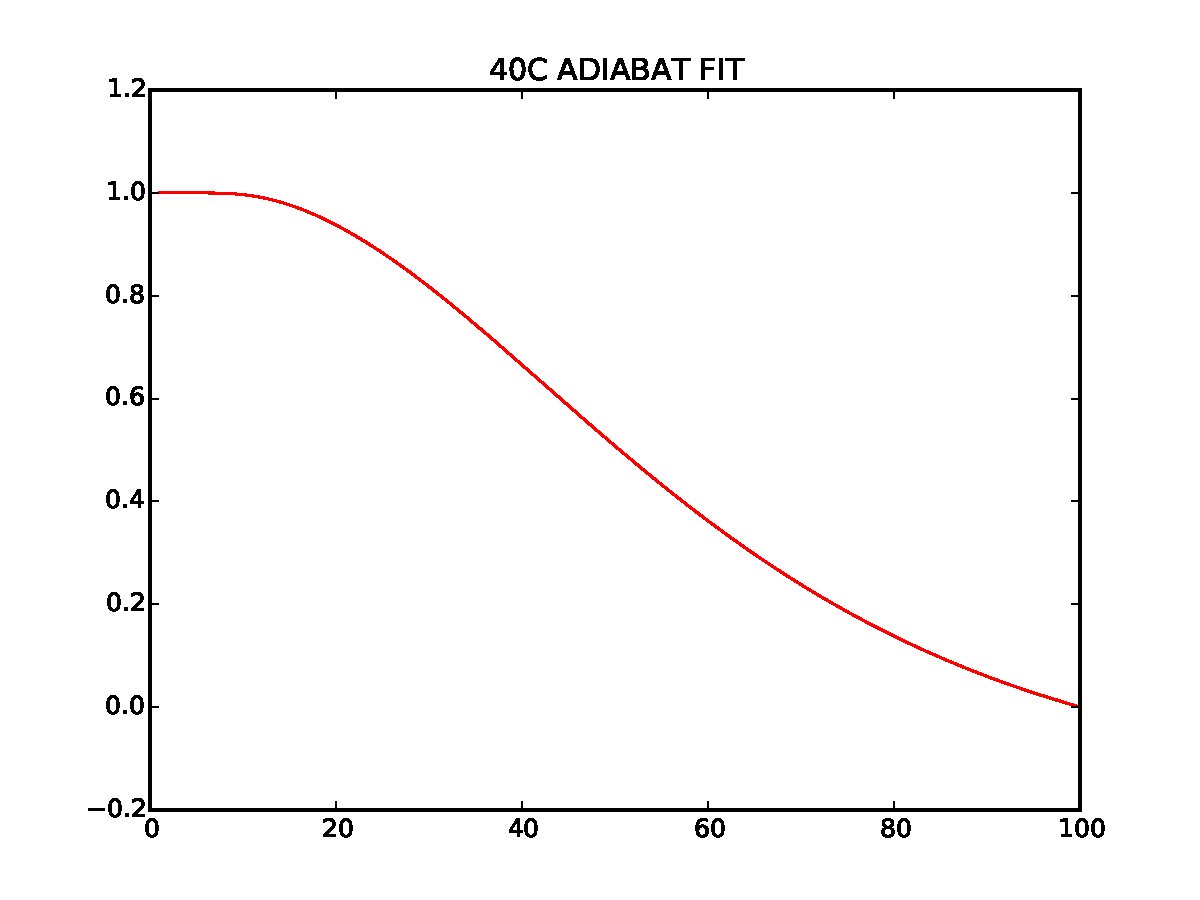
\includegraphics[width=4.5in]{../figs/pref_fit.pdf}
\caption{True and modelled $P_{ref} = +40C$ (difference between curves not apparent at this scale).}\label{pref}
\end{figure}

The next step is to choose a single functional form, which could represent the entire family of curves in Fig.\ref{trans_adiabats}. Each given shape of a particular curve is then controlled by variable parameters of the same function. A number of simple functions exist, which are able to model the relationship. For this work bi-exponential, arctan, rational and polynomial functions were tested. Generally, a reasonable fit can be achieved with both bi-exponential and arctan functions using as little as three variable parameters. While efficient, the results of such fit are unlikely to be sufficiently accurate to be useful. Another concern with these choices, is that the the variable parameters are not well-behaved functions and are hence difficult to model. 

Polynomial fitting doesn't appear to suffer from such issues. Moreover, the degree of accuracy can be controlled by increasing the degree of the polynomial and, hence, allowing a higher number of variable parameters. In this example, the curves were modelled using 8th degree polynomials, resulting in 9 variable parameters. Conveniently, and unlike other functional forms mentioned above, these parameters are also well-behaved. They can, again, be modelled using high-degree polynomials to the desired level of accuracy. Fig.\ref{fit_params} shows the results of parameter fitting for this given example. A demanding threshold of $MAE<1x10^{-6}$ was chosen for this example, and achieved using polynomial degrees of 17-24 (depending on the particular parameter).

\begin{figure}
\centering
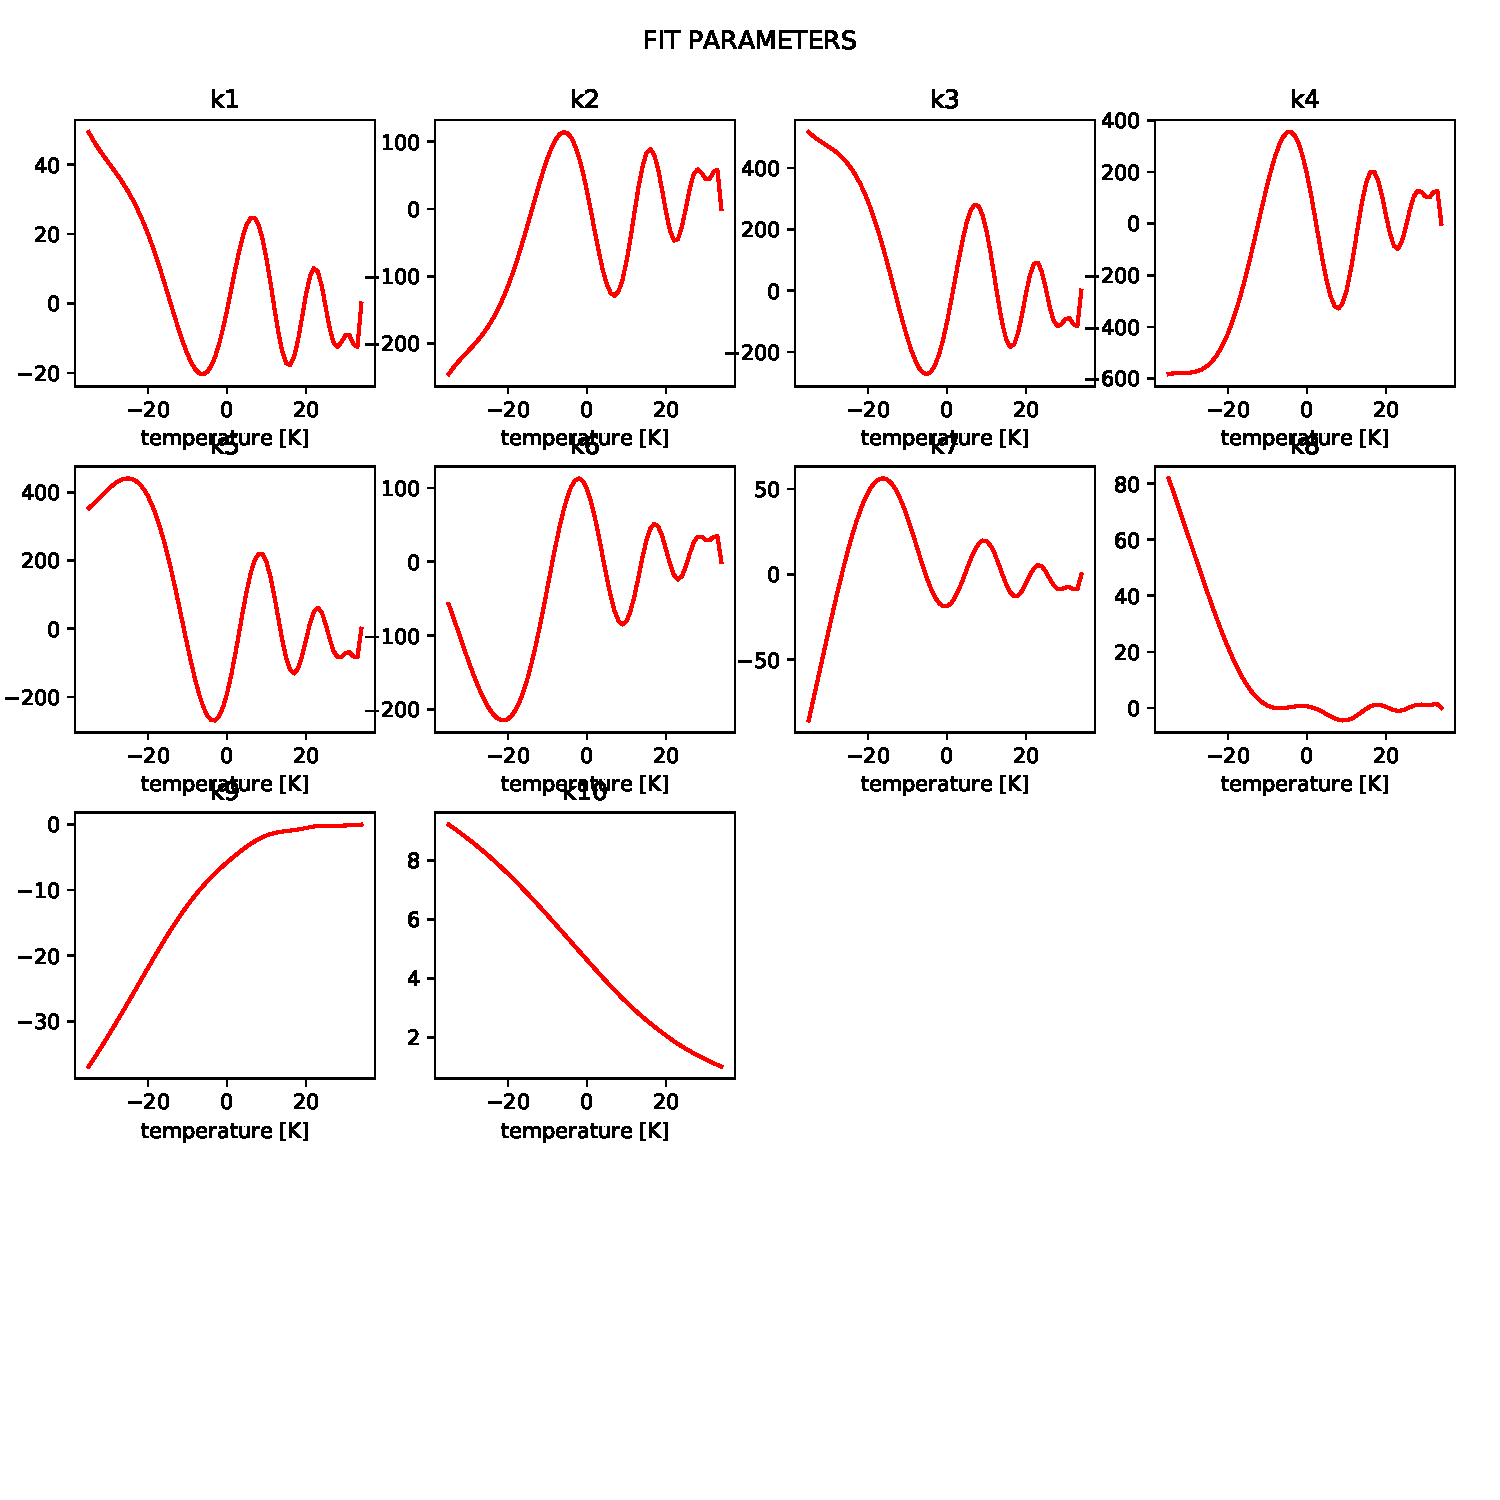
\includegraphics[width=7in]{../figs/fit_params.pdf}
\caption{True and modelled polynomial parameter fitting (difference between curves not apparent at this scale).}\label{fit_params}
\end{figure}

\FloatBarrier

\section*{Error Testing}

To test the accuracy of the proposed method, the moist adiabats can be modelled using the analytical approach and subsequently compared to those produced by direct iterative computation. For given $\Theta_w$, parameters $k1-k9$ in Fig.\ref{fit_params} are calculated using corresponding polynomial functions. For given $P$, $P_{ref}$ is derived using it's own polynomial relationship (Fig.\ref{pref}). Finally, normalized moist theta is calculated using 8th degree polynomial for given $P_{ref}$ and parameters $k1-k9$. The results are shown in Fig.\ref{final_fit}.

\begin{figure}
\centering
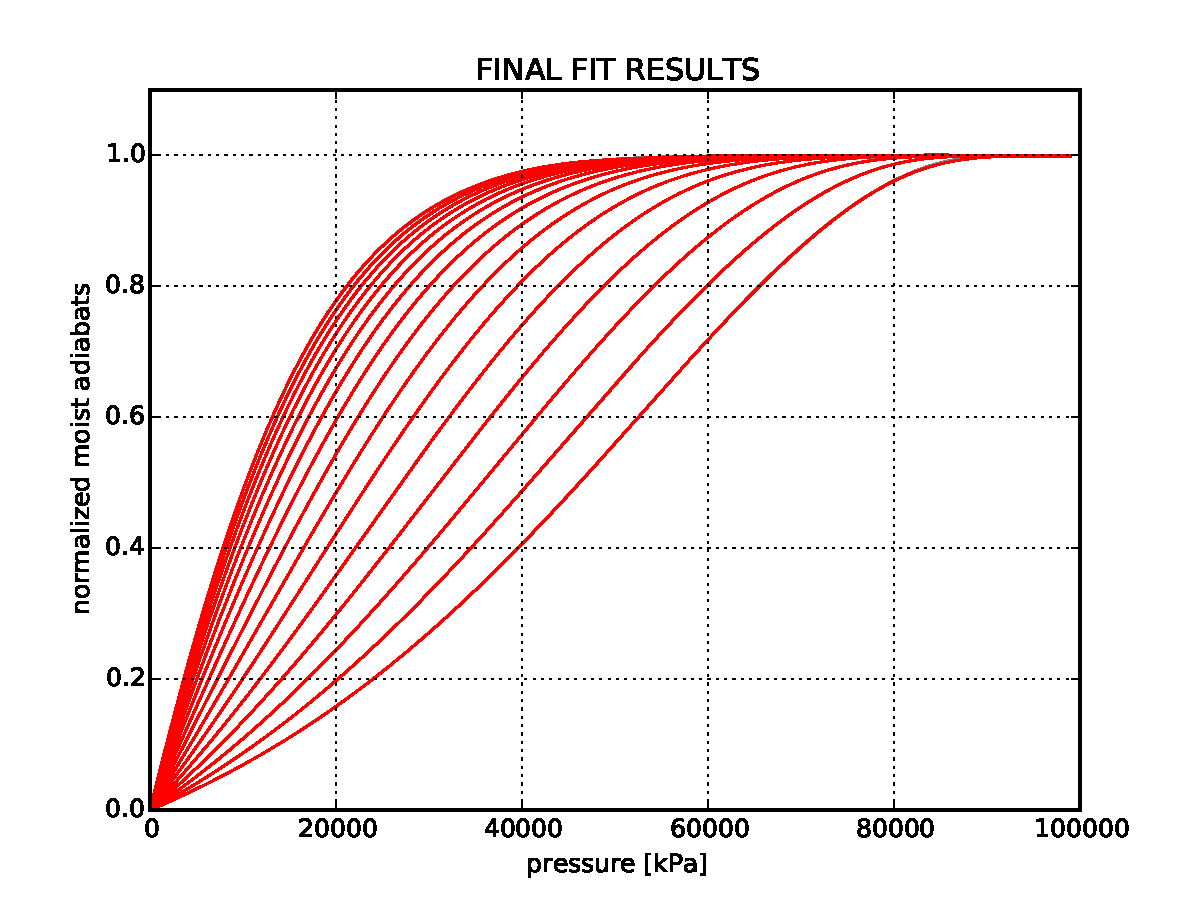
\includegraphics[width=4.5in]{../figs/final_fit.pdf}
\caption{True and modelled normalized moist theta (difference between curves not apparent at this scale). Select curves shown.}\label{final_fit}
\end{figure}

As mentioned earlier, higher accuracy may be achieved given the willingness to use even higher degrees of polynomials for fits. This is as effective as it is inelegant. For the current example the mean error profile for all 80 modelled adiabats is shown in Fig.\ref{error}.

\begin{figure}
\centering
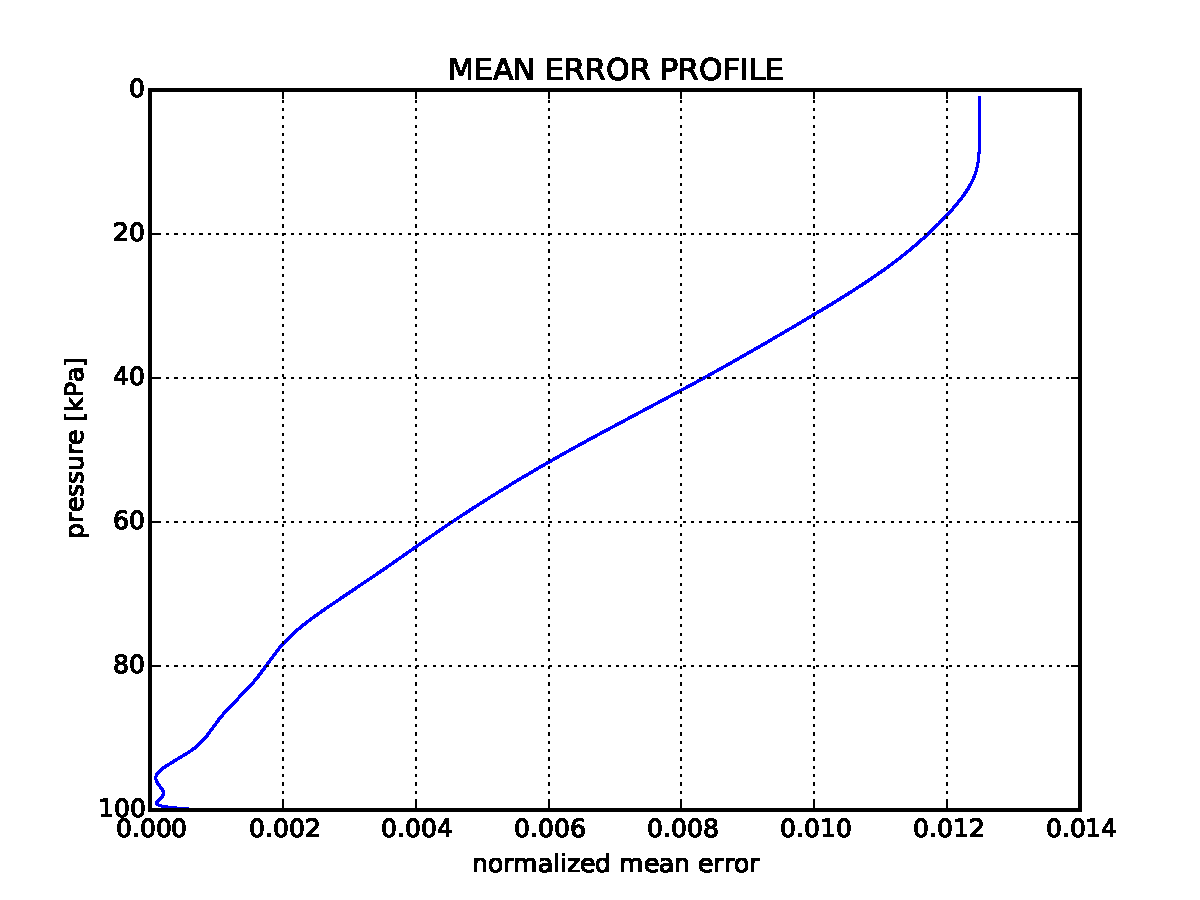
\includegraphics[width=4.5in]{../figs/error_profile.pdf}
\caption{Vertical mean error profile.}\label{error}
\end{figure}

\end{document}